\documentclass[11pt,a4paper]{article}
\usepackage{iftex}
\ifPDFTeX
  \usepackage[T1]{fontenc}
\fi
\usepackage[turkish,shorthands=:!]{babel}
\usepackage[margin=1.6cm]{geometry}
\usepackage{amsmath,amssymb}
\usepackage{multicol}
\usepackage{enumitem}
\usepackage{tikz}
\usetikzlibrary{babel,angles,quotes,calc}
\usepackage{pgfplots}
\pgfplotsset{compat=1.18}

\setlength{\columnsep}{1cm}
\setlength{\columnseprule}{0.4pt}
\pagestyle{empty}

% \begin{soru} ... \end{soru} — numaralı soru; metin, şekil ve şıklar
% sütun/sayfa sonunda bölünmeden aynı blokta kalır.
\newcounter{soru}
\newenvironment{soru}
  {\stepcounter{soru}\par\medskip\noindent
   \begin{minipage}{\linewidth}\textbf{\thesoru.}~\ignorespaces}
  {\end{minipage}\par\medskip}
% \siklar{A}{B}{C}{D}{E}    — kısa şıklar, tek satırda
% \siklaralt{A}{B}{C}{D}{E} — uzun şıklar, alt alta
\newcommand{\siklar}[5]{%
  \par\smallskip\noindent
  \makebox[0.2\linewidth][l]{A)~#1}\makebox[0.2\linewidth][l]{B)~#2}%
  \makebox[0.2\linewidth][l]{C)~#3}\makebox[0.2\linewidth][l]{D)~#4}%
  \makebox[0.2\linewidth][l]{E)~#5}\par}
\newcommand{\siklaralt}[5]{%
  \begin{enumerate}[label=\Alph*), leftmargin=2em, itemsep=1pt, topsep=2pt]
    \item #1 \item #2 \item #3 \item #4 \item #5
  \end{enumerate}}

\begin{document}

\begin{center}
  {\large\textbf{2026--2027 EĞİTİM ÖĞRETİM YILI}}\\[2pt]
  {\large\textbf{..... LİSESİ 10. SINIF MATEMATİK DERSİ 1. DÖNEM 1. YAZILI}}\\[8pt]
  \begin{tabular}{@{}l@{\hspace{3cm}}l@{}}
    Adı Soyadı: \rule{5cm}{0.4pt} & Numarası: \rule{2.5cm}{0.4pt} \\[4pt]
    Sınıfı: \rule{2cm}{0.4pt} & Puanı: \rule{2.5cm}{0.4pt}
  \end{tabular}
\end{center}
\hrule\medskip

\begin{multicols}{2}

\begin{soru}
Şekildeki $ABC$ üçgeninde $[CH] \perp [AB]$, $|AH| = 3$ birim, $|HB| = 5$ birim ve $|CH| = 4$ birimdir. Buna göre $|BC|$ kaç birimdir?
\begin{center}
  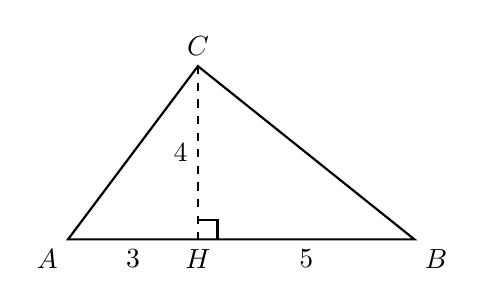
\begin{tikzpicture}[scale=0.55, thick]
  \coordinate (A) at (0,0);
  \coordinate (H) at (3,0);
  \coordinate (B) at (8,0);
  \coordinate (C) at (3,4);
  \draw (A) -- (B) -- (C) -- cycle;
  \draw[dashed] (C) -- (H);
  \pic[draw, angle radius=2.5mm] {right angle = C--H--B};
  \node[below left] at (A) {$A$};
  \node[below] at (H) {$H$};
  \node[below right] at (B) {$B$};
  \node[above] at (C) {$C$};
  \node[below] at (1.5,0) {$3$};
  \node[below] at (5.5,0) {$5$};
  \node[left] at (3,2) {$4$};
\end{tikzpicture}
\end{center}
\siklar{$\sqrt{34}$}{$6$}{$\sqrt{41}$}{$7$}{$\sqrt{57}$}
\end{soru}

\begin{soru}
Grafiği verilen $f(x) = x^2 - 2x - 3$ fonksiyonunun tepe noktasının koordinatları toplamı kaçtır?
\begin{center}
  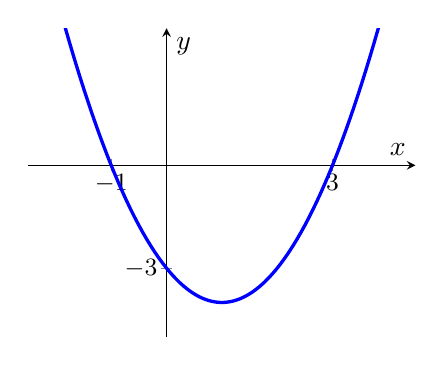
\begin{tikzpicture}
  \begin{axis}[
    axis lines=middle, xlabel={$x$}, ylabel={$y$},
    xmin=-2.5, xmax=4.5, ymin=-5, ymax=4,
    xtick={-1,3}, ytick={-3},
    width=6.5cm, height=5.5cm,
    every tick label/.append style={font=\small, fill=white, inner sep=1pt},
  ]
    \addplot[very thick, blue, domain=-1.9:3.9, samples=80] {x^2 - 2*x - 3};
  \end{axis}
\end{tikzpicture}
\end{center}
\siklar{$-5$}{$-3$}{$-1$}{$1$}{$3$}
\end{soru}

\begin{soru}
$2x - 1 \le 5$ eşitsizliğini sağlayan kaç farklı pozitif tam sayı vardır?
\siklar{$1$}{$2$}{$3$}{$4$}{$5$}
\end{soru}

\begin{soru}
Bir torbada 3 mavi ve 2 kırmızı top vardır. Torbadan iade edilmeden çekilen iki topun ikisinin de mavi olma olasılığı kaçtır?
\siklar{$\frac{1}{10}$}{$\frac{1}{5}$}{$\frac{3}{10}$}{$\frac{2}{5}$}{$\frac{3}{5}$}
\end{soru}

\end{multicols}

\vfill
\begin{center}\small Başarılar dileriz. \quad Süre: 40 dakika\end{center}

\end{document}
